\begin{fullwidth}
    \section{Overviewing dYdX Chain} \label{sec:introduction}

    \begin{adjustwidth}{2cm}{2cm}
        \justify
        The dYdX ecosystem is migrating to dYdX Chain with the launch of dYdX v4. dYdX Chain is a Cosmos blockchain built on the Cosmos SDK using the CometBFT consensus protocol. The chain's validators will operate its order book and matching engine, gossiping orders between each other and including transactions in new blocks when two orders are matched. With dYdX v4, all components of the dYdX protocol stack are decentralized, including the front end, indexers, order book, matching engine, and governance. Before diving into the ecosystem's migration, and the future responsibilities of the dYdX community, we first provide a brief overview of some components of dYdX Chain. Those knowledgeable about dYdX Chain might choose to skip to Section \ref{sec:migration}: The dYdX Chain Migration.
    \end{adjustwidth}
    
    \textcolor{gray}{\rule{\linewidth}{0.1mm}}
    
\end{fullwidth}

    dYdX v3 was an Ethereum L2 derivatives exchange built using the StarkEX engine. dYdX Trading, the team behind the dYdX protocol, maintained the exchange's order book and matching engine off-chain, with the StarkEX engine submitting transactions on-chain when orders were matched. This made dYdX v3 a hybrid between a centralized and decentralized exchange. It was decentralized in the sense that users custody their own assets, but it was centralized in that a trusted 3rd party intermediated all transactions.
    
    With the advent of dYdX v4, the entire protocol will be operated in a decentralized fashion, with responsibilities shared across dYdX governance, the chain's validators, front end operators, and indexer operators. For a primer on dYdX v4, read \bhref{https://dydx.exchange/blog/dydx-chain}{this} announcement from dYdX Trading!\sidenotequote{Most people don’t remember this, but dYdX was the \#1 DEX by volume in early 2020 by a lot. At times we were approaching 50\% market share. We were doing ~\$10m trade volume / day at the time.}{\bhref{https://antonio-dydx.medium.com/the-history-of-dydx-so-far-68bf46789f86}{The History of dYdX (so far)}, by Antonio Juliano, CEO dYdX}

    \subsection{First, What is dYdX?}

        dYdX is a decentralized financial (DeFi) protocol purpose-built for trading perpetual futures contracts for major cryptocurrencies, including BTC, ETH, SOL, and many more. dYdX allows users to interact with advanced financial instruments without the need for traditional intermediaries, thus providing more transparent and efficient financial system.

        With v3, dYdX emerged as one of the most successful DeFi platforms in the industry, driving billions of dollars in trading volume on a daily basis. Despite its significant success over the last few years, dYdX v3 will be deprecated in favor of the new and improved dYdX v4.

        We briefly overview the various features that differentiate dYdX v4 from it's previous Ethereum L2 implementation, and from other decentralized derivatives exchanges. Following this background information, we dive into the ecosystem's migration in the next section.
        
    \subsection{Off-Chain Order Book and Matching Engine}

        \begin{marginfigure}
            \centering
            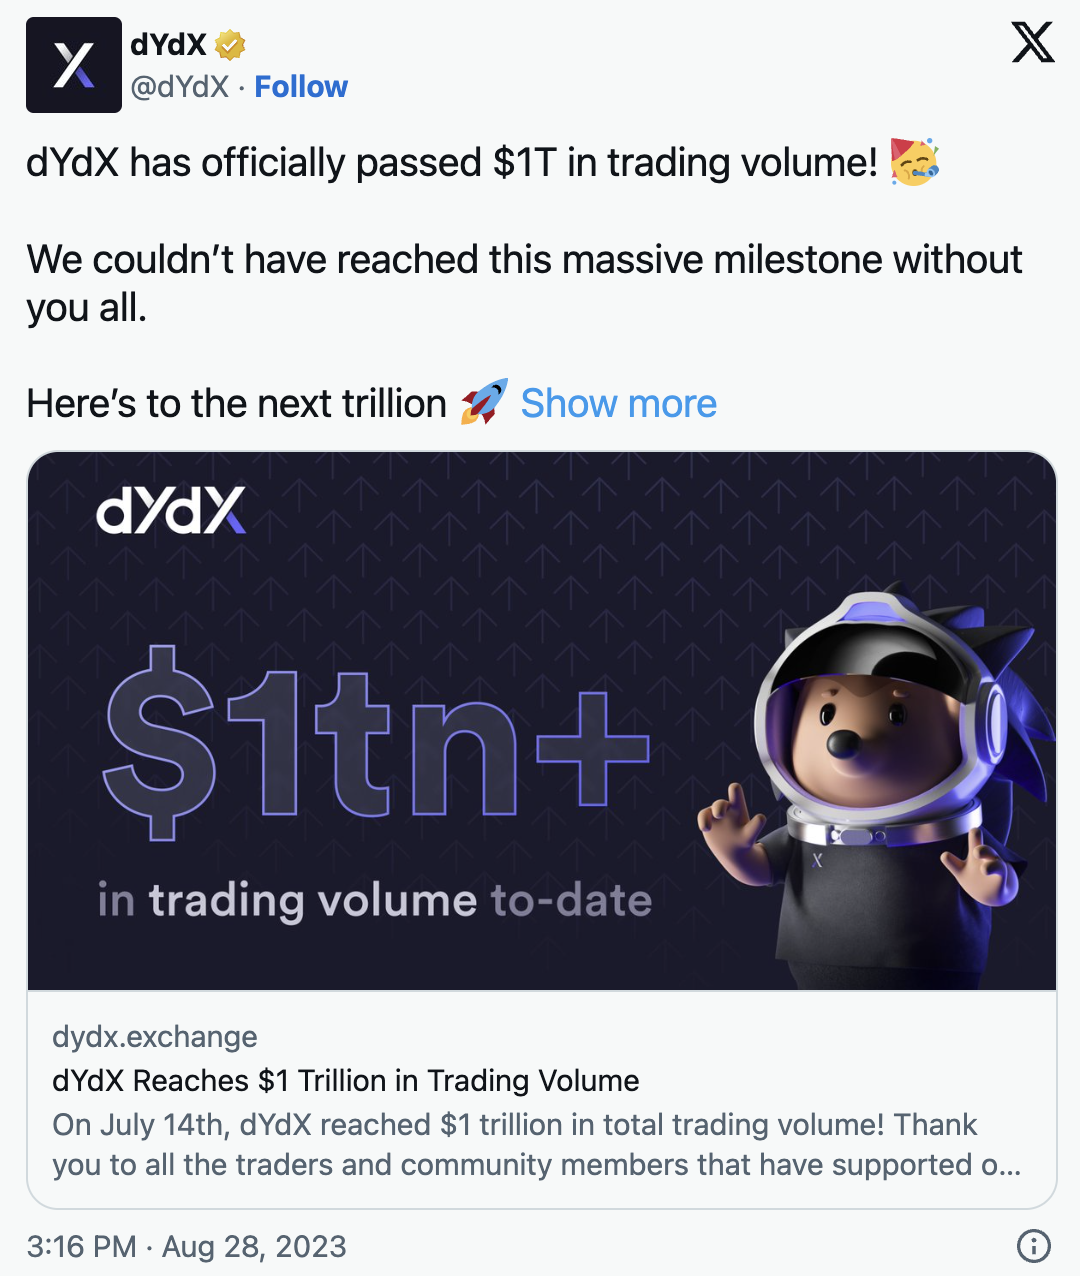
\includegraphics[width=\linewidth]{figs/trading_vol_tweet.png}
            \caption{ \bhref{https://x.com/dYdX/status/1696240239700852801?s=20}{Tweet} from @dYdX on crossing \$1 Trillion dollars in trading volume.}
            \label{fig:trading_vol_tweet}
        \end{marginfigure}
        
        A major benefit of developing a Cosmos blockchain, and a key innovation of dYdX v4, is that dYdX Chain's validators will operate an off-chain, in-memory order book and accompanying matching engine. An order book is a data structure that contains every user's intent to buy or sell an asset at a particular price, whereas a matching engine is the logic that matches a willing buyer with a willing seller. On dYdX Chain, validators constantly ``gossip'' orders between each other to ensure they each hold a roughly consistent version of the order book (not accounting for network latency). When two orders intersect, all validators run the same logic (the matching engine) to determine that the dYdX Chain must be updated with a new transaction, which is included by the block proposer in the next block.
        
        Notice that there are two main types of data packets that the protocol must track: orders and transactions. Orders are an intent to buy or sell an asset at a specific price, and are submitted and cancelled very frequently, on the order of 1000 orders per second. Transactions, on the other hand, track the exchange of an asset from one account to another when two orders are matched, updating the blockchain's state. Transactions occur less frequently, on the order of 10 transactions per second (TPS). 

        Since orders occur very frequently, and don't require a modification to anyone's account balances, it is unnecessarily burdensome to commit them to the chain during the consensus process. An off-chain order book and matching engine avert this problem, enabling dYdX to significantly increase its throughput. That is, dYdX Chain will be able to support more orders and more transactions (higher TPS) than alternative L1 and L2 solutions, without having any centralized 3rd party operating the order book and matching engine. According to several announcements from dYdX, this is a key reason for building on Cosmos.\sidenotequote{Trusting code instead of corporates has become more important in times of regulatory uncertainty and corporate failures. dYdX is lighthouse example on how transparency empowers the community to decide about the future, leading to safety, fairness, and equality. The development of a Decentralized Autonomous Organization (DAO) is a cornerstone of dYdX’s vision for decentralized governance and the community renewed its support the operations DAO. Further, the transition to dYdX Chain is one more step towards democratization of access to financial opportunities. }{\bhref{https://dydx.foundation/blog/dydx-2023-semi-annual-ecosystem-report}{Markus Spillman, dYdX Council Member}}

        This creates a more decentralized and transparent financial system, without sacrificing scalability and product quality, with the caveat that one must still trust the chain's validators to behave honestly. More on that in section \ref{subsec:mev}.

    \subsection{Cosmos Proof-of-Stake: Validators and Stakers}
    
        In Cosmos, validators are the key agents that keep a network running smoothly using the CometBFT Proof-of-Stake (PoS) consensus protocol. The active validator set is determined by a validator's staked DYDX, both self-staked and delegated from other users. If validators misbehave, part of their stake, or collateral, may be slashed and burnt\sidenote[][2cm]{This slashing is determined by a slashing parameter controlled by governance, and is set to 0 at Genesis.}. Cosmos chains, including dYdX Chain, derive their economic security from the value of this collateral, and the assumption that validators are incentivized to behave honestly and not get slashed.
        
        A validator's influence is not solely determined by their own staked tokens. A significant portion of their staking power comes from regular users, or ``stakers'' who delegate their tokens to a validator they trust. In return, stakers earn a share of the transaction fees generated by the network, and share the same slashing risks as the validators; if a validator acts dishonestly, both can lose part or all of their staked tokens.
        
        In the specific case of dYdX Chain, stakers hold the majority of the staked tokens, which makes them important decision-makers in the governance process. We will be referring to voters on dYdX Chain as ``stakers'' throughout this report.
        
        The governance model in Cosmos and dYdX v4 is different from earlier systems like dYdX v3. In the latter, any token holder could vote on proposals. In contrast, in Cosmos and dYdX v4, the primary voting power lies with the validators. Stakers inherit their validator's decision unless they actively choose to vote differently. Importantly, this means that token holders that don't stake their tokens on the chain cannot influence the governance process.
        
    \subsection{Gas and Trading Fees}

        By building on Cosmos, dYdX may also customize when and how users pay gas fees. Similar to dYdX v3, there are no gas fees to submit or cancel orders, partly because doing so does not require an update to the blockchain's state. Instead, users only pay trading fees when orders are matched and assets are exchanged. These fees accrue to the chain's validators and stakers based on the validators' commission rates, and the stakers' shares of the chain's overall stake. As of now, these trading fees are paid in the collateral asset, USDC.
        
        Additionally, the community may eventually activate a ``Community Tax'' on all trading fees, which it may then leverage to fund ecosystem growth or pay service providers. At genesis, the community tax will be set to 0\%. More on trading fees and the community tax in section \ref{sec:validators}. 

    \subsection{Technical Stack Overview}

        \begin{figure}[htp]
            \centering
            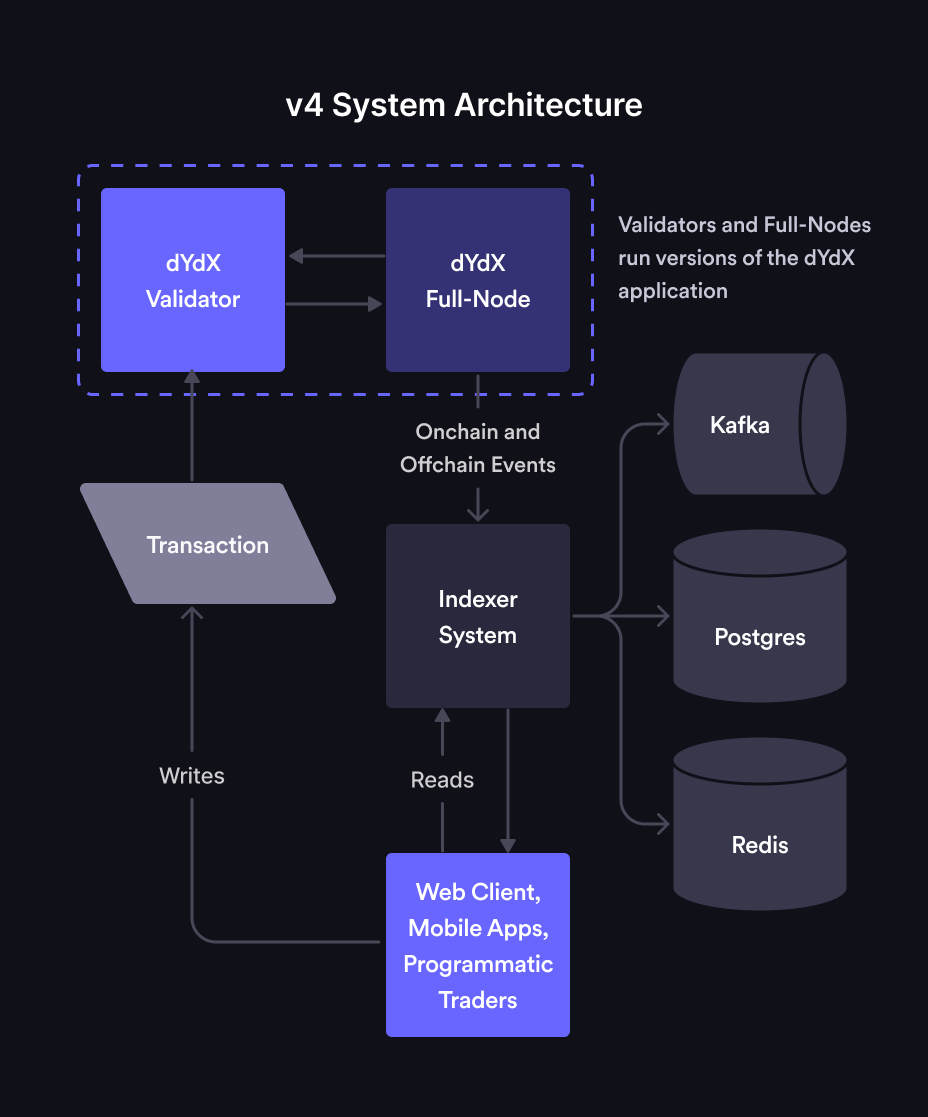
\includegraphics[width=0.5\linewidth]{figs/V4_System_Architecture__1_.png}
            \caption{The v4 System architecture, taken from the \bhref{https://dydx.exchange/blog/v4-technical-architecture-overview}{v4 Technical Architecture Overview} blog post.}
            \label{fig:architecture}
        \end{figure}

        Throughout this report we will refer to a few components of dYdX Chain's technical stack. This includes the software run by the Chain's validators, as well as the indexers and front ends that support the Chain. At a high-level, the Indexer system allows API users and front-ends to query the current state of the protocol, including the off-chain order book. This is what allows the front-end to display the shape and depth of the order book, and compute relevant quantities such as slippage. The front-end is a user interface that allows retail users to access the dYdX protocol without writing any code, and is available both on the web and on mobile systems such as Android and iOS. We will discuss the front end in depth on Section \ref{sec:feip}, and what incentives might be put in place to get operators to deploy a variety of front ends.

        The entire technical stack for operating dYdX Chain, from its matching engine, to its front ends have been open-sourced by dYdX Trading, on their public GitHub \bhref{https://github.com/dydxprotocol}{page}. For a deeper understanding of the Chain's architecture, refer to \bhref{https://dydx.exchange/blog/v4-technical-architecture-overview}{this} blog post.

    \subsection{Native USDC Collateral, Bridging, and IBC}

        \begin{marginfigure}
            \centering
            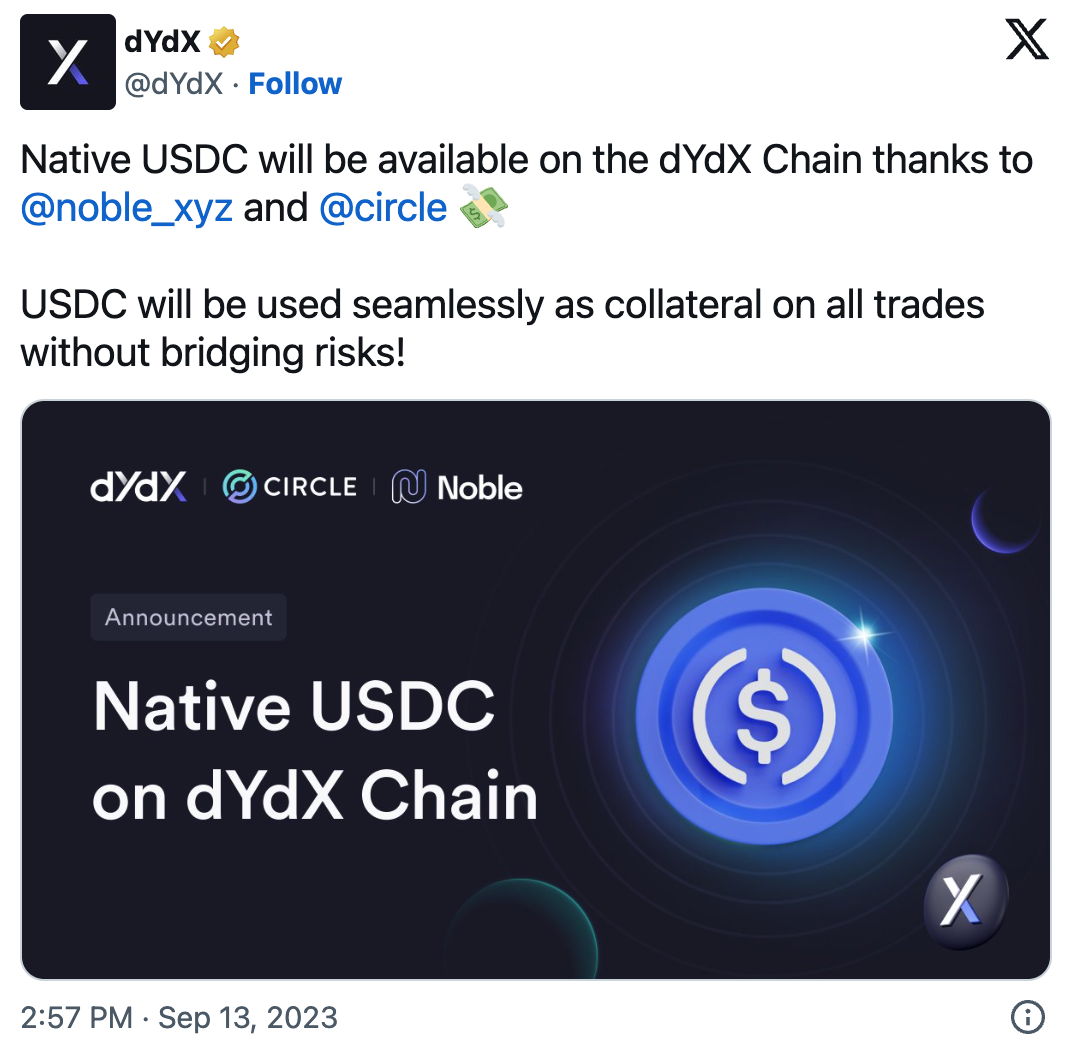
\includegraphics[width=\linewidth]{figs/usdc_announcement.png}
            \caption{dYdX Announces native USDC will be used as collateral on dYdX Chain, powered by \bhref{https://nobleassets.xyz/}{Noble.xyz}.}
            \label{fig:usdc_announcement}
        \end{marginfigure}

        On dYdX v3 all positions are collateralized by USDC, which is minted on Ethereum. A natural question might be, how will positions on dYdX Chain be collateralized, and will this incur some bridging risk? 
        
        Recently, dYdX, Circle, and Noble have announced that USDC will launch natively on Cosmos, powered by the Noble blockchain. This native USDC may then be used on dYdX Chain via the Inter-Blockchain Communication (IBC) protocol, which carries different and fewer security assumptions than many other L1 - L1 bridging solutions.

        Aside from depositing into dYdX Chain using native USDC from Noble, dYdX users may also bridge USDC from Ethereum and its many roll-ups to dYdX Chain in \bhref{https://dydx.exchange/blog/1-click-onboarding}{one click}! This is done with the support of Squid, a transaction builder built on top of the Axelar protocol.

    \subsection{An Aside On Cosmos}
        
        We will not go into depth on how Cosmos works in this report, and we will assume the reader has some basic knowledge of the Cosmos SDK and the Tendermint protocol. Please refer to the Cosmos SDK or Tendermint documentation if there is any confusion, or to \bhref{https://dydx.forum/t/dydx-v4-a-beginners-guide-to-cosmos/761}{this} detailed guide to Cosmos put together by RoboMcGobo, a dYdX and Osmosis contributor.

    % \subsection{DYDX Emissions Schedule} \label{subsec:emissions}

    %     Throughout this report we refer to several expenses that affect the distribution of DYDX token from the dYdX community's treasuries (namely the community treasury and rewards treasury). We provide the emissions schedule for DYDX as of September 2023 for reference in Fig. \ref{fig:emissions}. Notice the emissions schedule encompasses the community's recurring expenses, and does not include one-off expenses such as funding the dYdX Operations Trust or the dYdX Grants Program.

    %     \begin{figure}[htp]
    %         \centering
    %         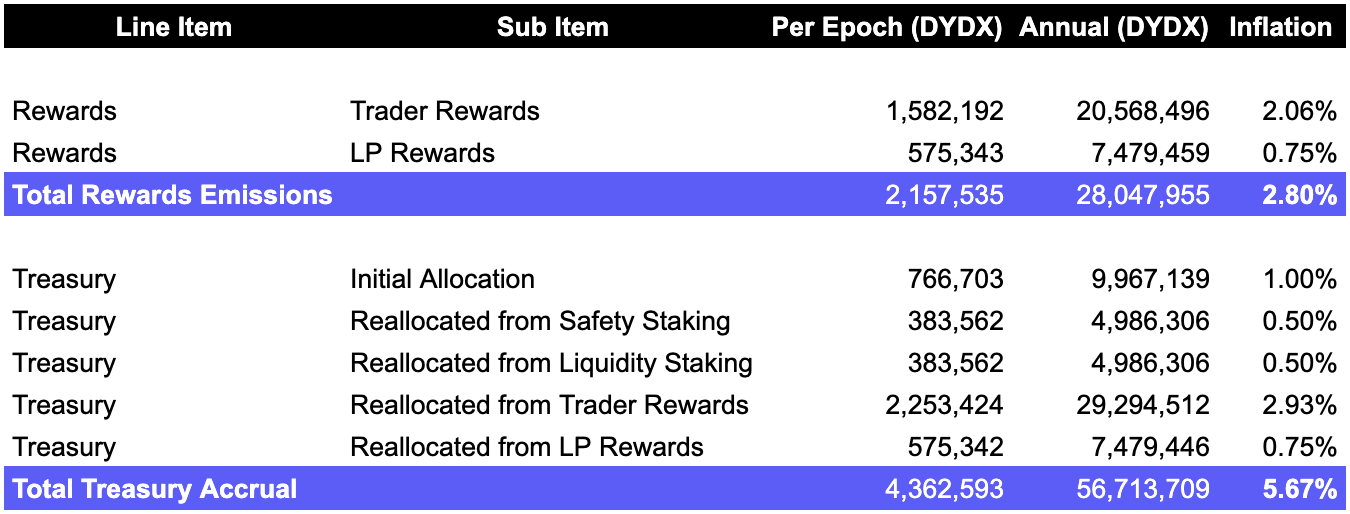
\includegraphics[width=0.8\linewidth]{figs/emissions.png}
    %         \caption{DYDX Emissions on dYdX v3 as of September 2023.}
    %         \label{fig:emissions}
    %     \end{figure}

    %     As of September 2023, the DYDX vesting schedule is set to conclude on August 2026, at which point no more DYDX will vest into either the community or rewards treasuries. Once the original vesting concludes, dYdX governance may choose to enact a maximum 2\% annual inflationary schedule. 

    %     \begin{figure}[htp]
    %         \centering
    %         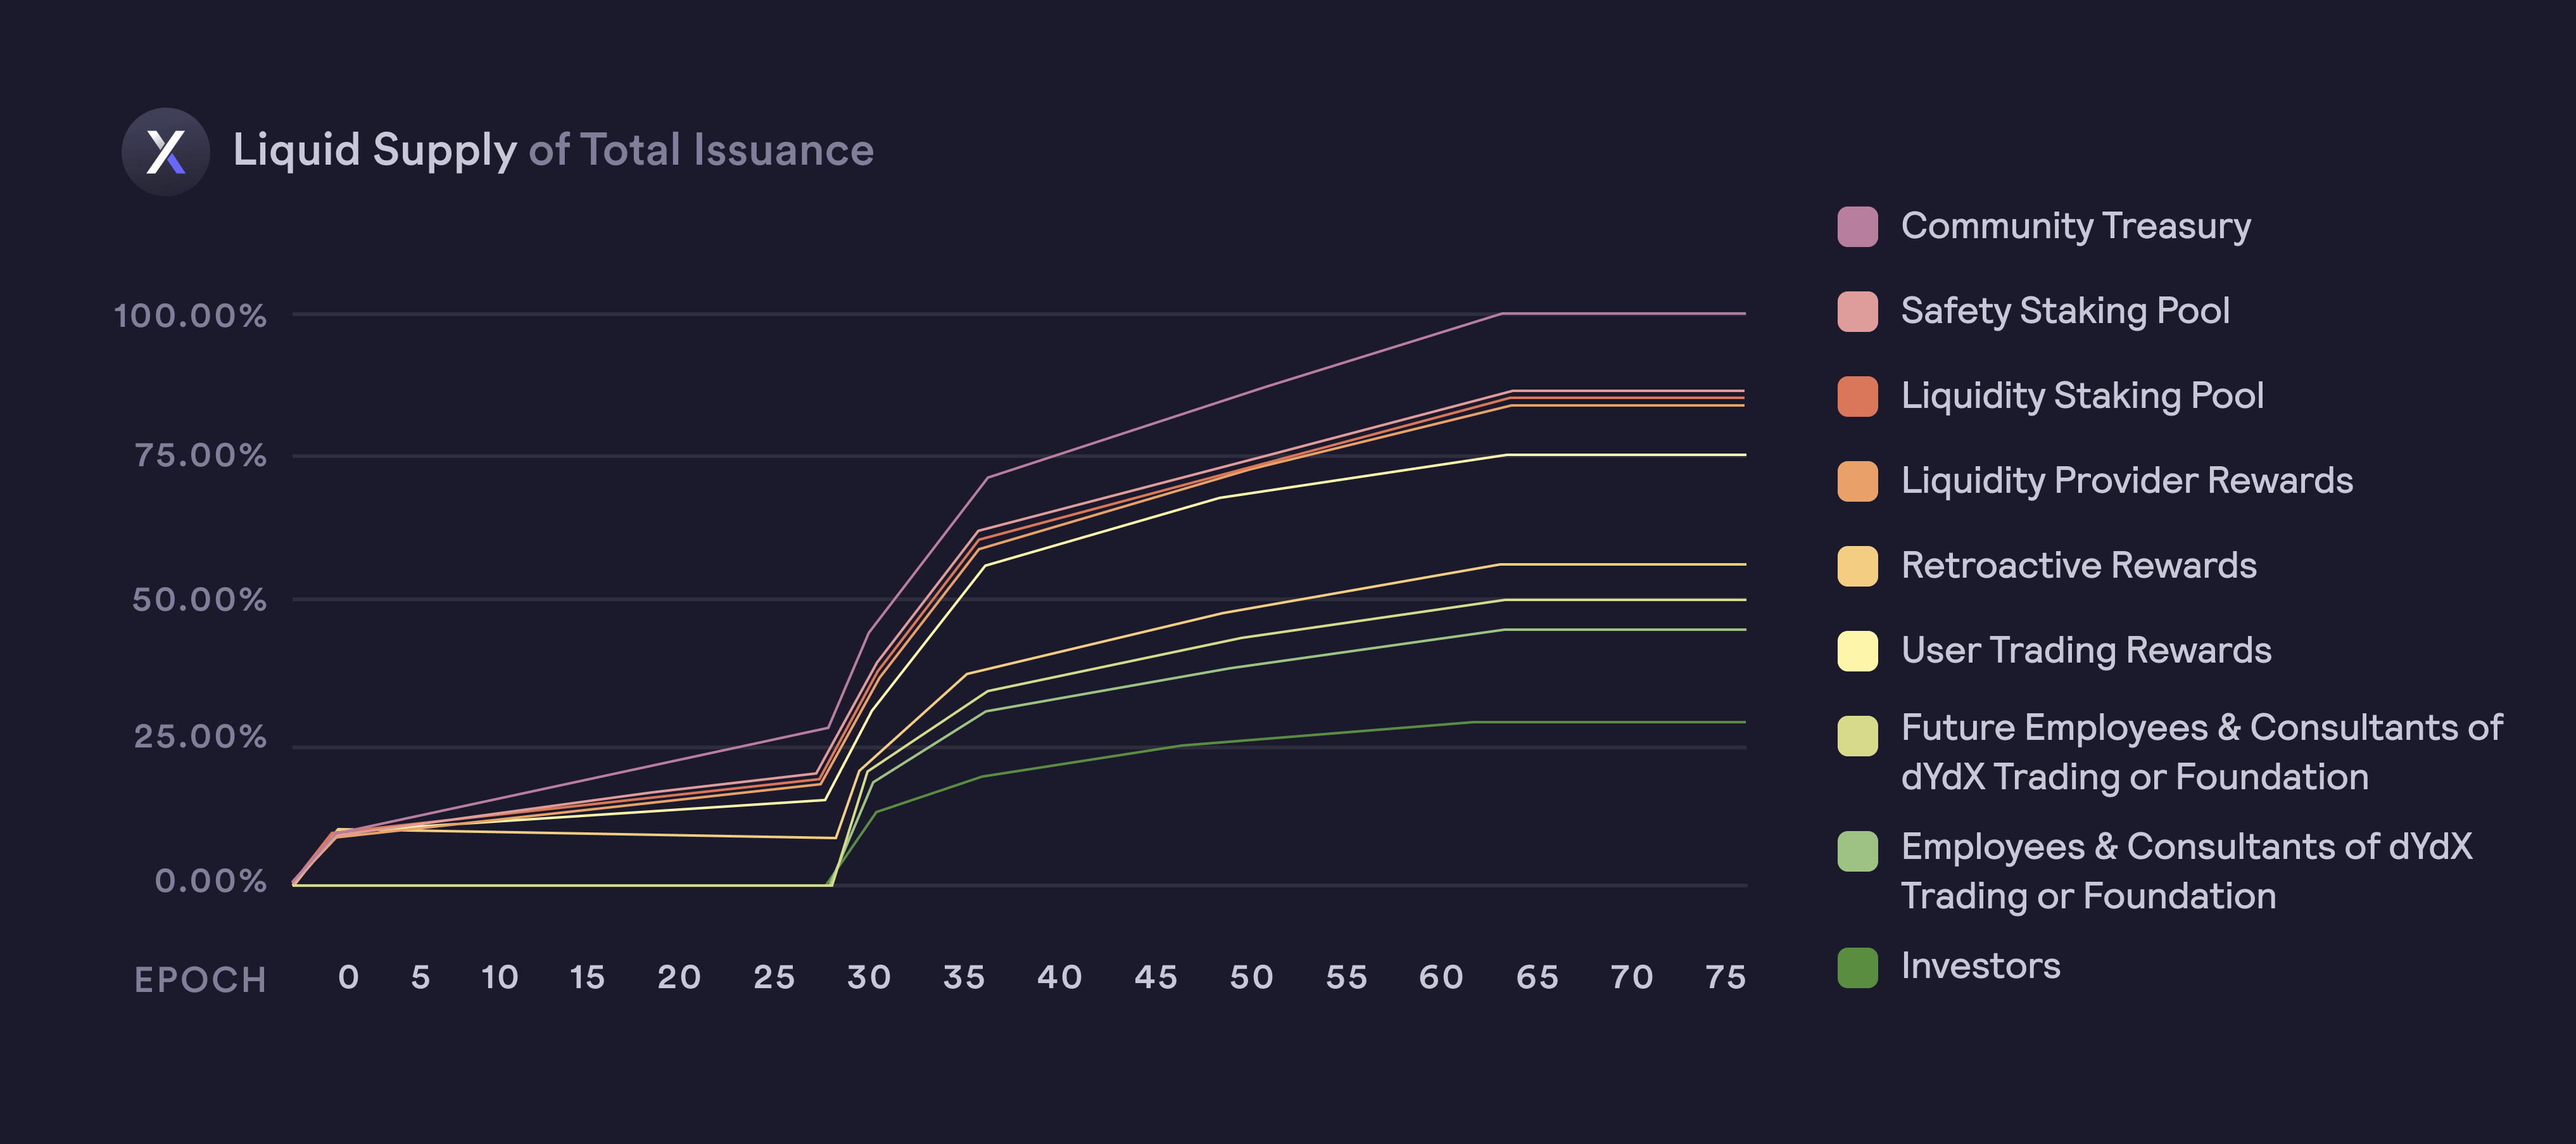
\includegraphics[width=0.8\linewidth]{figs/vesting.png}
    %         \caption{DYDX token vesting schedule.}
    %         \label{fig:vesting}
    %     \end{figure}